\subsection{Decentralized approach}
The simulation is carried out setting the step size $\alpha(k) = \frac{0.001}{k+1}$. The termination condition is met when the aggregated power profile is under the threshold $P^{max}_i$ and is within $30 kW$ of the minimum between $P^{max}_i$ and the reference $P^{ref}_i$.

Figure \ref{fig:dec_stop_criterion} shows the amount of maximum violation of the global constraint and the maximum deviation between the solution and the reference (regarding the maximum aggregated power). In particular, for small values of k (i.e., the initial iterations of the algorithm) the PEVs try to greedily impose a (globally unfeasible) charging schedule. As the iterations proceed, the central controller modifies the Lagrange multipliers $\lambda$, $\mu$, $\nu$ in order to force the convergence to a feasible solution, which is reached after $17$ iterations. As a matter of fact, that is when the termination condition is met.

The aggregated power profile solution is shown in Figure \ref{fig:dec_power}. Notice that it always satifies the global constraint, even though it is not as faithful to the reference as the centralized solution. This is due to the fact that the PEVs do not have access to the global information.


\begin{figure}[H]
    \centering
    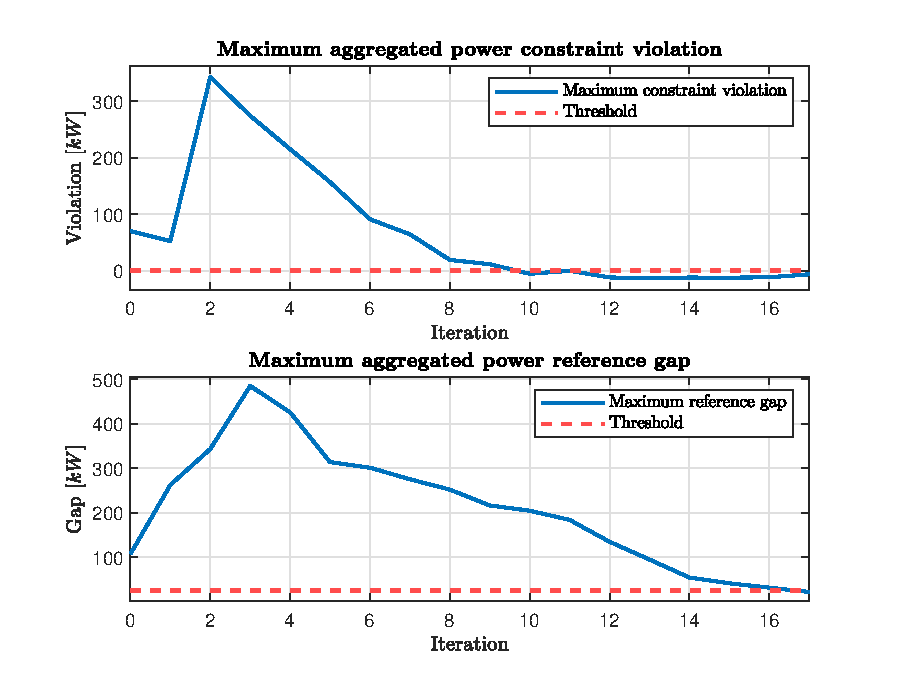
\includegraphics[width=\columnwidth]{figures/images/stop_criterion.eps}
    \caption{Maximum global constraint violation and maximum deviation from the adjusted reference per iteration of the decentralized algorithm.}
    \label{fig:dec_stop_criterion}
\end{figure}

\begin{figure}[H]
    \centering
    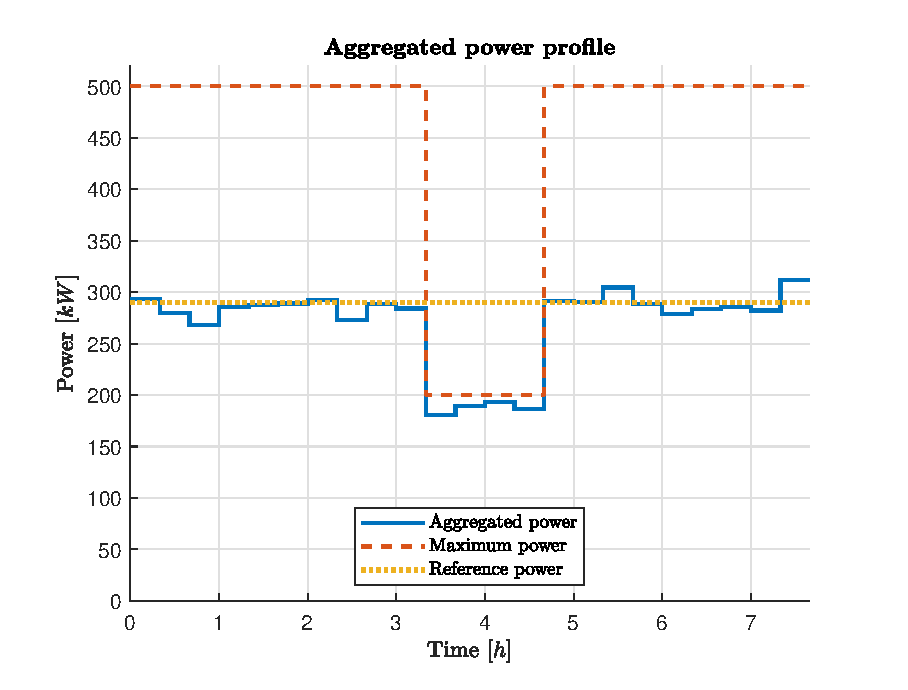
\includegraphics[width=\columnwidth]{figures/images/dec_power.eps}
    \caption{Aggregated power profile of the PEVs in the decentralized case.}
    \label{fig:dec_power}
\end{figure}

\begin{figure}[H]
    \centering
    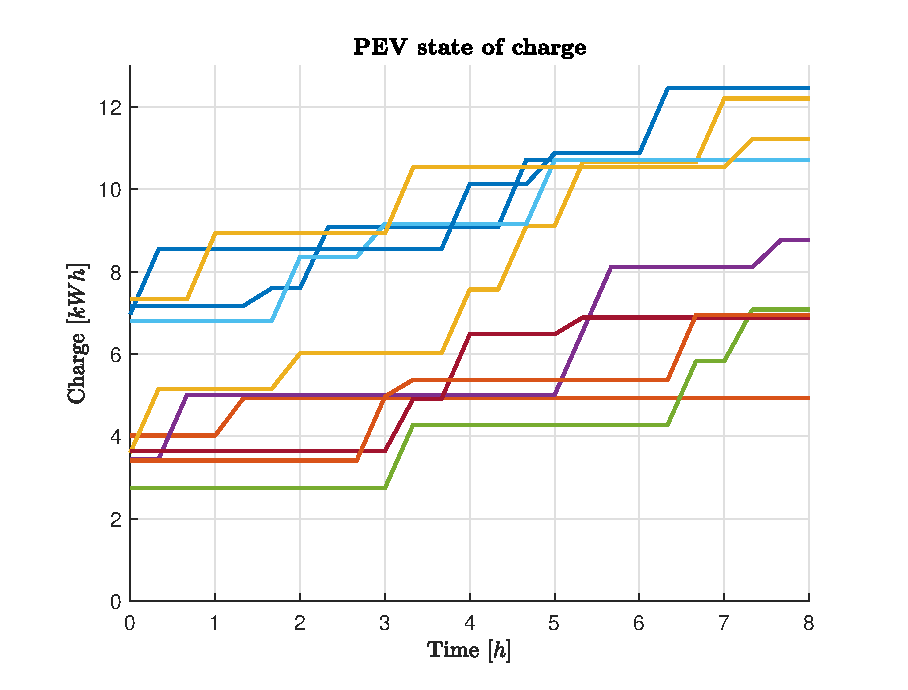
\includegraphics[width=\columnwidth]{figures/images/dec_state.eps}
    \caption{State of charge evolution of the PEVs in the decentralized case.}
    \label{fig:dec_state}
\end{figure}


Figure \ref{fig:dec_state} displays the state of charge of a random batch of 10 PEVs. As in the centralized case, the charging process is carried out correctly.

The evolution of $||\rho_p||_2$ can be analyzed in Figure \ref{fig:dec_rho} accordingly to line 9 of Algorithm \ref{algo:dec}. The increase of the magnitude of $\rho_p$ goes hand in hand with the approach to the globally feasible optimal solution (compare with Figure \ref{fig:dec_stop_criterion}).

Finally, in Figure \ref{fig:dec_multipliers} the consequent progression of the multipliers is displayed. Iteration after iteration, they are updated according to lines 11-13 of Algorithm \ref{algo:dec}, and they play a crucial role in the computation of the solutions of the inner optimization problems (line 5). In fact, since in the first iterations the global constraints are violated, the multipliers mutate in order to force the convergence to a feasible solution. 
\begin{figure}[H]
    \centering
    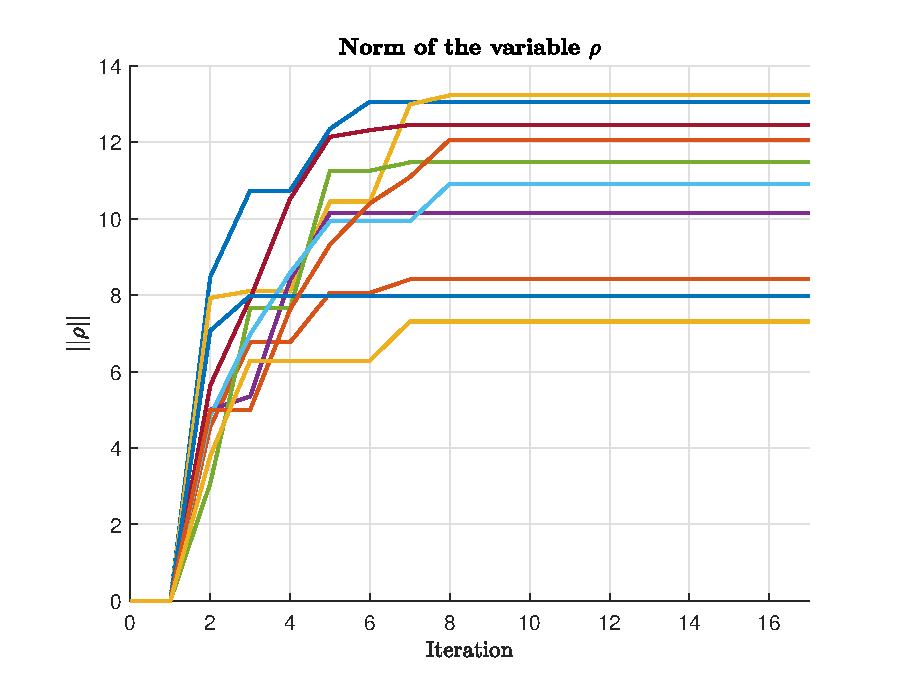
\includegraphics[width=\columnwidth]{figures/images/rho.eps}
    \caption{Norm of $\rho$ for a random batch of $10$ PEVs per iteration of the decentralized algorithm.}
    \label{fig:dec_rho}
\end{figure}


In terms of computational burden, there is a significant improvement with respect to the centralized approach. By averaging the time that each PEV takes to solve the inner optimization problem, we get $0.159\,s$. Hence, to carry out 17 iterations, the algorithm takes about $2.7\,s$.
\end{multicols}
\begin{figure}[H]
    \center
    \begin{minipage}{5.4cm}
        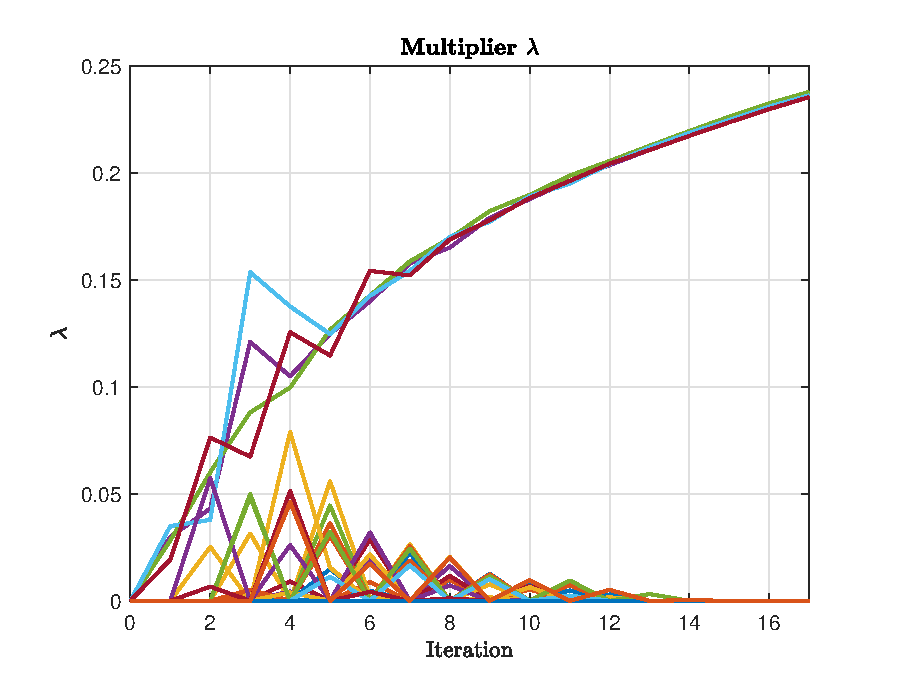
\includegraphics[width=\columnwidth]{figures/images/lambda.eps}
    \end{minipage}
    \begin{minipage}{5.4cm}
        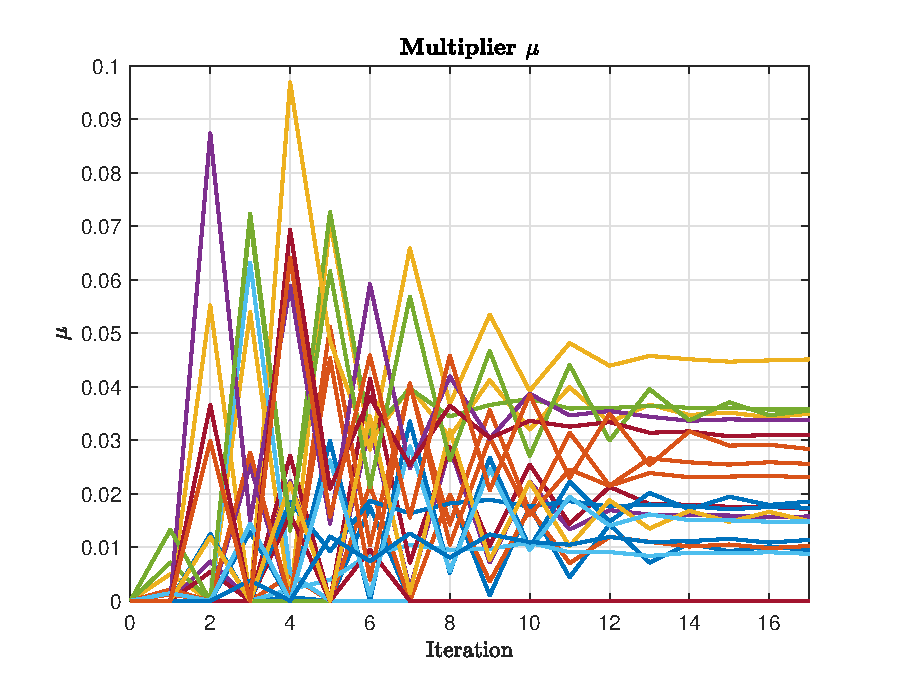
\includegraphics[width=\columnwidth]{figures/images/mu.eps}
    \end{minipage}
    \begin{minipage}{5.4cm}
        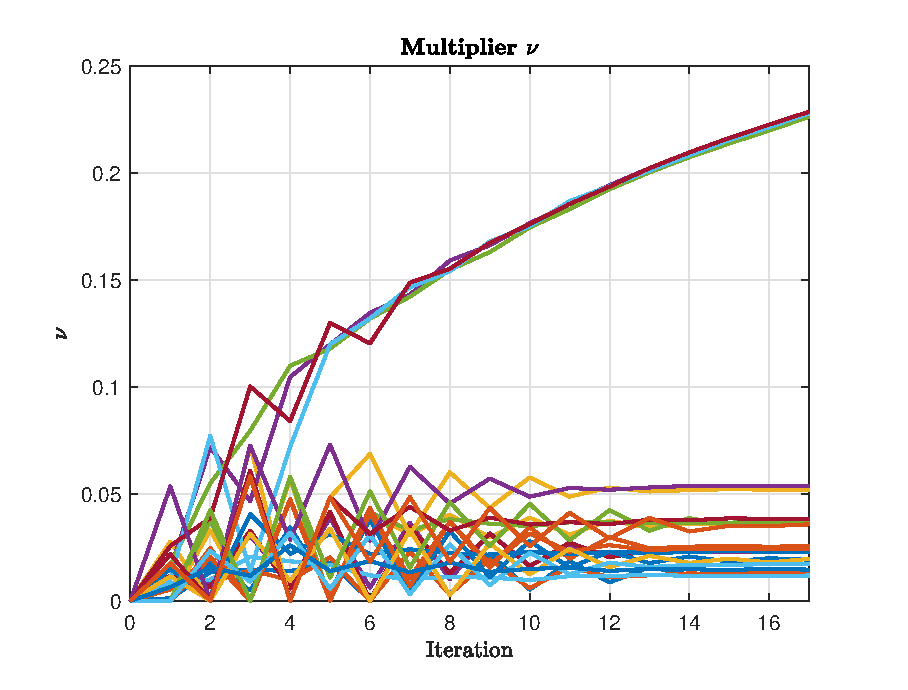
\includegraphics[width=\columnwidth]{figures/images/nu.eps}
    \end{minipage}
    \caption{Evolution of the Lagrange multipliers per iteration of the decentralized algorithm.}
    \label{fig:dec_multipliers}
\end{figure}
\begin{multicols}{2}